% Saving this styling, because "Kvant" pages set it to their own
\newcommand{\labstyling}{
    \newgeometry{
        top=2cm,
        bottom=2cm,
        inner=2cm,
        outer=2cm
    }
    
    \changefontsize{13pt}

    % Positioning page-numbers for lab
    \pagestyle{fancy}
    \fancyhf{}
    \fancyfoot[C]{\thepage}
    \renewcommand{\headrulewidth}{0pt} % Because of fancyhdr, a line appears at the top of the page
}
\labstyling

\begin{titlepage}
   \begin{center}
        Федеральное государственное автономное \\
        образовательное учреждение высшего образования \\
        «Национальный исследовательский университет ИТМО» \\
        Факультет Программной Инженерии и Компьютерной Техники \\
        
        \vspace{2cm}
    
        \begin{large}
            Лабораторная работа № 6 \\
            по дисциплине \\
            "Информатика"
                
            \vspace{1.5cm}
    
            Вариант №3
        \end{large}

        \vfill
       
        \begin{flushright}
            \textbf{Выполнил:} \\
            Студент группы P3130, \\
            Гусяков Ратмир Кириллович
        \end{flushright}
        \begin{flushright}
            \textbf{Проверил:} \\
            Балакшин Павел Валерьевич
        \end{flushright}
        
        \vspace{0.5cm}
        Санкт-Петербург \\
        2022
            
   \end{center}
\end{titlepage}

\tableofcontents

\clearpage

\section{Подготовка к заданию}

\begin{enumerate}
    \item Скачать и установить любой дистрибутив TEX (например, MiKTeX) или создать аккаунт на сайте ShareLaTeX (\url{sharelatex.com}), Overleaf (\url{overleaf.com}) или любом аналогичном.
    
    \item Выбрать год и номер журнала \guillements{Квант} (\url{kvant.ras.ru}) согласно варианту из таблицы на последней странице документа. Вариант выбирается как сумма последнего числа в номере группы, умноженного на 10, и номера в списке группы согласно ISU на текущий день.
    
    \item Выбрать одну страницу из всего номера, отвечающую следующим требованиям:
        \begin{itemize}
            \item Текст должен состоять минимум из 2 колонок.
            
            \item Заголовок не должен превышать 20\% от площади страницы.
            
            \item Страница должна содержать 1 или 2 картинки, общая площадь которых не должна превышать 40\% площади страницы.
            
            \item Текст должен содержать не менее 2 сложных формул. Желательно, чтобы были такие математические операции, как сумма элементов (не путать с простым сложением), извлечение корня, логарифм и т.п.
            
            \item В тексте должна быть как минимум 1 таблица. Размерность таблицы должна превышать 2*2 элемента.
        \end{itemize}
        В случае, если такая страница не найдена, то взять 1.5 страницы, где на одной будет б\`{о}льшая часть задания, а на оставшейся – меньшая. 
        
        В случае, если и таким образом страница не найдена, необходимо увеличить год выпуска на 19 лет и искать материал в новом выпуске
\end{enumerate} 

\section{Задание}

\subsection{Обязательное задание}

Сверстать страницу, максимально похожую на выбранную страницу из журнала
\guillements{Квант}.

\subsection{Необязательное задание}

\emph{Выполнение данного задания позволяет получить до 10 дополнительных процентов от максимального числа баллов БаРС за данную лабораторную}

\begin{enumerate}
    \item Сверстать титульный лист
    \item Создать файл \emph{main.tex}, в котором будет содержаться преамбула и ссылки на 2 документа: титульный лист и статью (ссылки создаются с помощью команды \verb|\input|).
\end{enumerate}

\subsection{Вариант}

\begin{figure}[!htb]
   \begin{minipage}{0.48\textwidth}
     \centering
     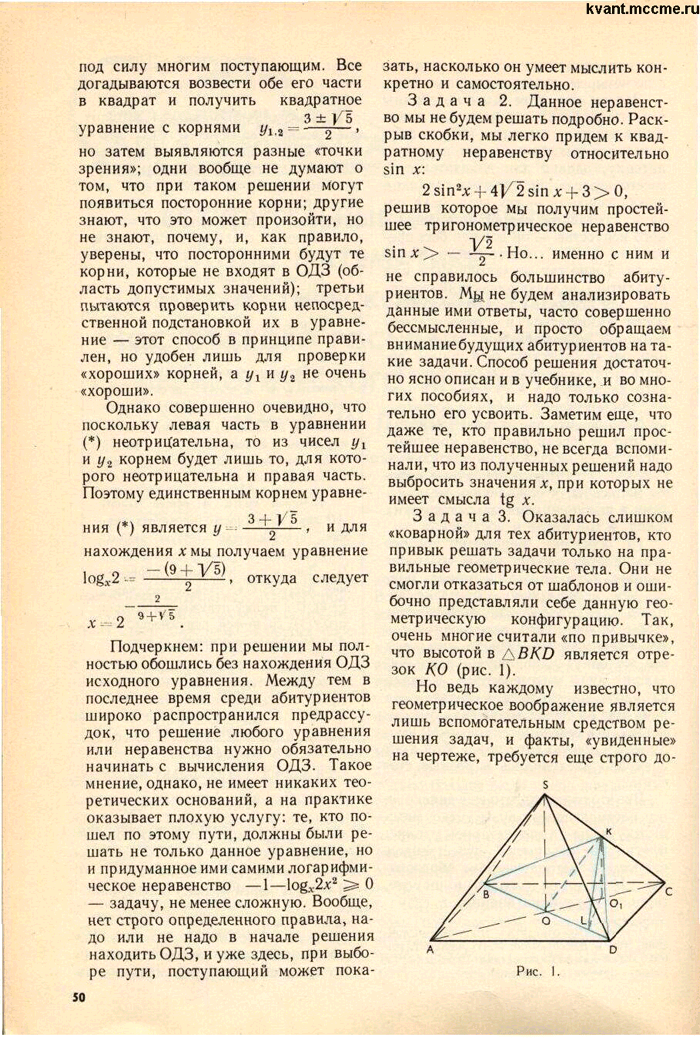
\includegraphics[width=.85\linewidth]{kvant_70_03-50.png}
     \caption{\footnotesize{50-я страница 3 номера 1970 года. Два столбца, математические формулы и картинка}}\label{fig:kvant-70-page}
   \end{minipage}\hfill
   \begin{minipage}{0.48\textwidth}
     \centering
     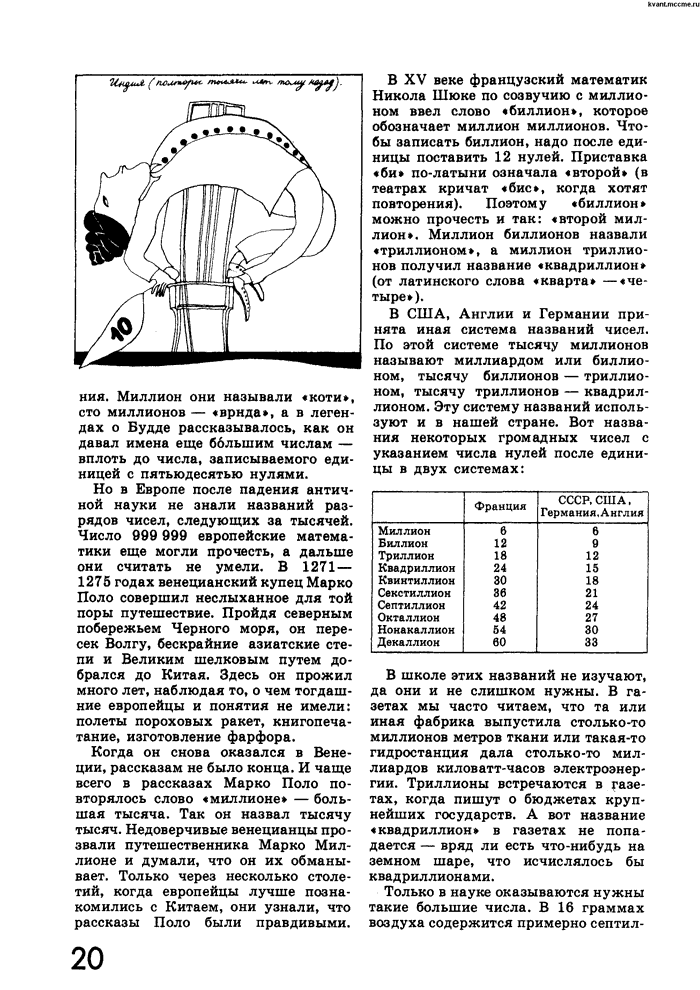
\includegraphics[width=.9\linewidth]{kvant_89_03-20.png}
     \caption{\footnotesize{20-я страница 3 номера 1989 года. Два столбца, картинка и таблица}}\label{fig:kvant-88-page}
   \end{minipage}
\end{figure}

\newpage

\section{Результат}

\subsection{Исходный код}

Исходный код со всеми фалами разметки и картинками: \newline
\url{https://github.com/B0nBun/InformaticsLab6}

\subsection{Итог}

Следующие 2 страницы представляют результаты верстки

\clearpage

\invisiblesubsubsection{\guillements{Квант} 1970-03-50}

% Setting all the margins and boxes
\newgeometry{
letterpaper,
top=1.5cm,
bottom=1.4cm,
footskip=0.1cm,
inner=2.5cm,
outer=1cm,
marginparwidth=0cm
}
\setlength{\columnsep}{30pt}

\changefontsize{13pt}

% Positioning page-numbers
\pagestyle{fancy}
\fancyhf{}
\fancyfoot[L]{\llap{\textbf{50}}} % \llap to move the number "out of bounds"
\renewcommand{\headrulewidth}{0pt} % Because of fancyhdr, a line appears at the top of the page

\begin{multicols}{2}
\noindent
под силу многим поступающим. Все догадываются возвести обе его части в квадрат и получить квадратное уравнение с корнями $y_{1,2} = \dfrac{3 \pm \sqrt{5}}{2}$, но затем выявляются разные \guillements{точки зрения}; одни вообще не думают о том, что при таком решении могут появиться посторонние корни; другие знают, почему, и, как правило, уверены, что посторонними будут те корни, которые не входят в ОДЗ (область допустимых значений); третьи пытаются проверить корни непосредственной подстановкой их в уравнение - этот способ в принципе правилен, но удобен лишь для проверки \guillements{хороших} корней, а $y_1$ и $y_2$ не очень \guillements{хороши}.

Однако совершенно очевидно, что поскольку левая часть в уравнении (*) неотрицательна, то из чисел $y_1$ и $y_2$ корнем будет лишь то, для которого неотрицательна и правая часть. Поэтому единственным корнем уравнения (*) является $y = \dfrac{3 + \sqrt{5}}{2}$, и для нахождения $x$ мы получаем уравнение $\log_x 2 = \dfrac{-(9 + \sqrt{5})}{2}$.

Подчеркнем: при решении мы полностью обошлись без нахождения ОДЗ исходного уравнения. Между тем в последнее время среди абитуриентов широко распространился предрассудок, что решение любого уравнения или неравенства нужно обязательно начинать с вычисления ОДЗ. Такое мнение, однако, не имеет никаких теоретических оснований, а на практике оказывает плохую услугу: те, кто пошел по этому пути, должны были решать не только данное уравнение, но и придуманное ими самими логарифмическое неравенство $-1 - \log_x{2x^2} \geq 0$ - задачу, не менее сложную. Вообще, не строго определенного правила, надо или не надо в начале решения находить ОДЗ, и уже здесь, при выборе пути, поступающий может показать, насколько он умеет мыслить конкретно и самостоятельно.

\setcounter{taskcounter}{2}
\task Данное неравенство мы не будем решать подробно. Раскрыв скобки, мы легко приведем к квадратному неравенству относительно $x$:

\centerline{$2\sin^{2}{x} + 4 \sqrt{2} \sin{x} + 3 > 0,$}

\noindent
решив которое мы получим простейшее тригонометрическое неравенство $\sin{x} > - \tfrac{\sqrt{2}}{2}$. Но... именно с ним и не справилось большинство абитуриентов. Мы не будем анализировать данные ими ответы, часто совершенно бессмысленные, и просто обращаем внимание будущих абитуриентов на такие задачи. Способ решения достаточно ясно описан и в учебнике, и во многих пособиях, и надо только сознательно его усвоить. Заметим еще, что даже те, кто правильно решил простейшее неравенство, не всегда вспоминали, что из полученных решений, не всегда вспоминали, что из полученных решений надо выбросить значения $x$, при которых не имеет смысла $\tg{x}$.

\task Оказалась слишком \guillements{коварной} для тех абитуриентов, кто привык решать задачи только на правильные геометрические тела. Они не смогли отказаться от шаблонов и ошибочно представляли себе данную геометрическую конфигурацию. Так, очень многие считали \guillements{по привычке}, что высотой в $\triangle BKD$ является отрезок $KO$ (рис. \ref{fig:70-triangle}).

Но ведь каждому известно, что геометрическое воображение является лишь вспомогательным средством решения задач, и факты, \guillements{увиденные} на чертеже, требуются еще строго до-

\begin{figure}[H]
    \hfill % Using horizontal filling because `right` argument for graphics doesn't work
    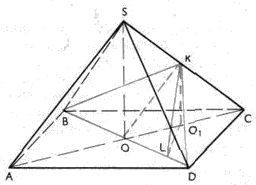
\includegraphics[width=.4\textwidth]{kvant_70-triangle-transparent.png}
    \caption{{}}
    \label{fig:70-triangle}
\end{figure}

\end{multicols}

\clearpage

\invisiblesubsubsection{\guillements{Квант} 1989-03-20}
% Setting all the margins and boxes
\newgeometry{
letterpaper,
top=2cm,
bottom=2cm,
footskip=1.5cm,
inner=2cm,
outer=2cm,
marginparwidth=0cm
}

\changefontsize{12pt}

% Positioning page-numbers
\pagestyle{fancy}
\fancyhf{}
\fancyfoot[L]{
    \selectlanguage{english}
    \fontfamily{qag}{\selectfont{
        \Huge 20
    }}
    \selectlanguage{russian}
}
\renewcommand{\headrulewidth}{0pt} % Because of fancyhdr, a line appears at the top of the page

\begin{multicols}{2}

\begin{figure}[H]
    \centering
    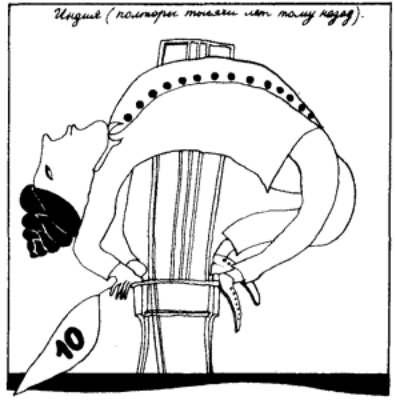
\includegraphics[width=0.9\linewidth]{kvant_89-lying.png}
    \label{fig:kvant_89-lying}
\end{figure}

\noindent ния. Миллион они называли \guillements{коти}, сто миллионов - \guillements{врнда}, а в легендах о Будде рассказывалось, как он давал имена еще б\`{о}льшим числам - плоть до числа, записываемого единицей с пятьюдесятью нулями.

Но в Европе после падения античной науки не знали  названий разрядов чисел, следующих за тысячей. Число 999 999 европейские математики еще могли прочесть, а дальше они считать не умели. В 1271-1275 годах венецианский купец Марко Поло совершил неслыханное для той поры путешествие. Пройдя северным побережьем Черного моря, он пересек Волгу, бескрайние азиатские степи и Великим шелковым путем добрался до Китая. Здесь он прожил много лет, наблюдая то, о чем тогдашние европейцы и понятия не имели: полеты пороховых ракет, книгопечатание, изготовление фарфора.

Когда он снова оказался в Венеции, рассказам не было конца. И чаще всего в рассказах Марко Поло повторялось слово \guillements{миллионе} - большая тысяча. Так он назвал тысячу тысяч. Недоверчивые венецианцы прозвали путешественника Марко Миллионе и думали, что он их обманывает. Только через несколько столетий, когда европейцы лучше познакомились с Китаем, они узнали, что рассказы Поло были правдивыми.

В XV веке французский математик Никола Шюке по созвучию с миллионом ввел слово \guillements{биллион}, которое означает миллион миллионов. Что бы записать биллион, надо после единицы поставить 12 нулей. Приставка \guillements{би} по-латыни означала \guillements{второй} (в театрах кричат \guillements{бис}, когда хотят повторения). Поэтому \guillements{биллион} можно прочесть и так: \guillements{второй миллион}. Миллион биллионов назвали \guillements{триллионом}, а миллион триллионов получил название \guillements{квадриллион} (от латинского слова \guillements{кварта} - \guillements{четыре}).

В США, Англии и Германии принята иная система названий чисел. По этой системе тысячу миллионов называют миллиардом или биллионом, тысячу биллионов - триллионом, тысячу триллионов - квадриллионом. Эту систему названий используют и в нашей стране. Вот названия некоторых громадных чисел с указанием числа нулей после единицы в двух системах:


\begin{table}[H]
    \centering
    \begin{tabular}{|l|c|c|}
         \hline
         \; & Франция & \thead{СССР, США, \\ Германия, Англия} \\
         \hline
         Миллион     & 6  & 6  \\
         Биллион     & 12 & 9  \\
         Триллион    & 18 & 12 \\
         Квадриллион & 24 & 15 \\
         Квинтиллион & 30 & 18 \\
         Секстиллион & 36 & 21 \\
         Септиллион  & 42 & 24 \\
         Окталлион   & 48 & 27 \\
         Нонакаллион & 54 & 30 \\
         Декаллион   & 60 & 33 \\
         \hline
    \end{tabular}
    \label{tab:millions_table}
\end{table}

В школе этих названий уже не изучают, да они и не слишком нужны. В газетах мы часто читаем, что та или иная фабрика выпустила столько-то миллионов метров ткани или такая-то гидростанция дала столько-то миллиардов киловатт-часов электроэнергии. Триллионы встречаются в газетах, когда пишут о бюджетах крупнейших государств. А вот название \guillements{квадриллион} в газетах не попадается - вряд ли есть что-нибудь на земном шаре, что исчислялось бы квадриллионами.

Только в науке оказываются нужны такие числа. В 16 граммах воздуха содержится примерно септил-

\end{multicols}


\clearpage

\labstyling

\section{Вывод}

В процессе выполнения этой лабораторной работы, я научился работать с основными механизмами системы разметки \LaTeX, такими как использование окружений, команд, создание макросов, счетчиков, вставка картинок, таблиц и т.д. Продемонстрировать же все эти умения мне удалось через копирование разметки журнала \guillements{Квант}.